\section{Анализ задания}
\label{sec:analys}

Оптическая скамья -- установка, представляющая из себя массивную направляющую с насаженными на нее рейтерами с оптическими элементами.
Рейтеры можно перемещать и неподвижно закреплять в любом ее месте при сохранении строгой параллельности оптическим и визирным осям.
\begin{figure}[!h]
    \centering
    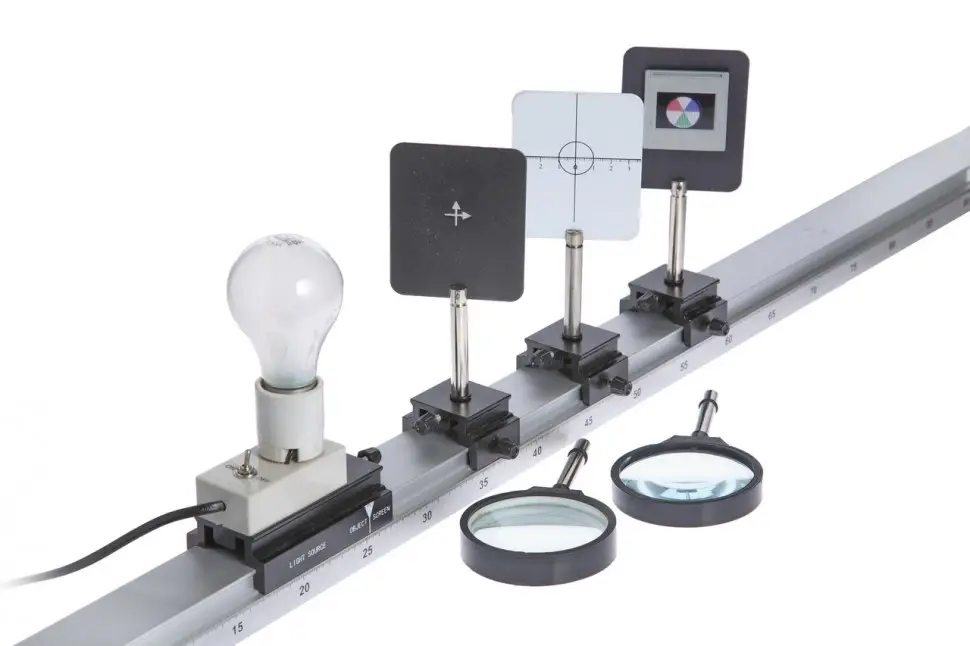
\includegraphics[width=0.5\textwidth]{img/img}
    \caption{Оптическая скамья с рейтерами}
    \label{fig:img}
\end{figure}

Необходимо разработать измерительное устройство для угловых перемещений зеркала относительно его горизонтальной оси.
Устройство должно обладать высокой точностью и относительно небольшим диапазоном измерения ($\pm5^\circ$), что необходимо учитывать при выборе метода измерения.
